\documentclass{standalone}
\usepackage{ctex}
\usepackage{tikz}
\usepackage{xcolor}
\usetikzlibrary{positioning,calc,arrows.meta,backgrounds}

\begin{document}
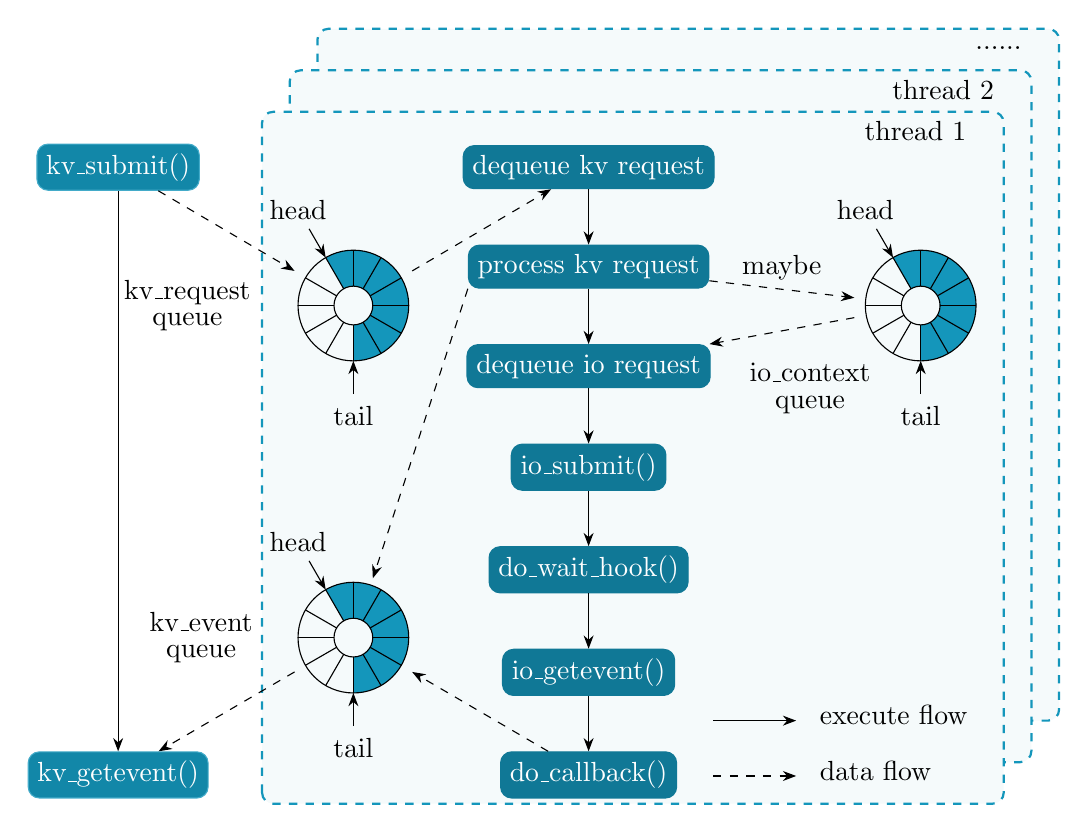
\begin{tikzpicture}[
    every node/.style={draw,node distance=2em,rounded corners,text=color5}
  ]
  \linespread{0.8}

  \definecolor{color1}{HTML}{107896}
  \definecolor{color3}{HTML}{1287a8}
  \definecolor{color2}{HTML}{1496bb}
  \definecolor{color4}{HTML}{43abc9}
  \definecolor{color5}{HTML}{ffffff}

  \node[fill=color1,draw=color1] at (0,0)          (worker1)  {dequeue kv request};
  \node[below=of worker1,fill=color1,draw=color1]  (worker2)  {process kv request};
  \node[below=of worker2,fill=color1,draw=color1]  (worker3)  {dequeue io request};
  \node[below=of worker3,fill=color1,draw=color1]  (worker4)  {io\_submit()};
  \node[below=of worker4,fill=color1,draw=color1]  (worker5)  {do\_wait\_hook()};
  \node[below=of worker5,fill=color1,draw=color1]  (worker6)  {io\_getevent()};
  \node[below=of worker6,fill=color1,draw=color1]  (worker7)  {do\_callback()};
  \draw[-Stealth] (worker1) -- (worker2);
  \draw[-Stealth] (worker2) -- (worker3);
  \draw[-Stealth] (worker3) -- (worker4);
  \draw[-Stealth] (worker4) -- (worker5);
  \draw[-Stealth] (worker5) -- (worker6);
  \draw[-Stealth] (worker6) -- (worker7);

  \coordinate (kv-que) at (-8.5em,-5em);
  \fill[color2] ($(kv-que)+(-90:0.7em)$) arc[start angle=-90,end angle=120,radius=0.7em] -- ++(120:1.3em) arc[start angle=120,delta angle=-210,radius=2em] -- cycle;
  \draw (kv-que) circle[radius=0.7em];
  \draw (kv-que) circle[radius=2em];
  \foreach \x in {0,30,...,330}
    \path ($(kv-que)+(\x:0.7em)$) -- ++(\x:1.3em)[draw];
  \node[draw=none,text=black] at ($(kv-que)+(120:4em)$)  {head};
  \node[draw=none,text=black] at ($(kv-que)+(-90:4em)$)  {tail};
  \draw[-Stealth] ($(kv-que)+(120:3.2em)$) -- ($(kv-que)+(120:2em)$);
  \draw[-Stealth] ($(kv-que)+(-90:3.2em)$) -- ($(kv-que)+(-90:2em)$);

  \coordinate (event-que) at (-8.5em,-17em);
  \fill[color2] ($(event-que)+(-90:0.7em)$) arc[start angle=-90,end angle=120,radius=0.7em] -- ++(120:1.3em) arc[start angle=120,delta angle=-210,radius=2em] -- cycle;
  \draw (event-que) circle[radius=0.7em];
  \draw (event-que) circle[radius=2em];
  \foreach \x in {0,30,...,330}
    \path ($(event-que)+(\x:0.7em)$) -- ++(\x:1.3em)[draw];
  \node[draw=none,text=black] at ($(event-que)+(120:4em)$)  {head};
  \node[draw=none,text=black] at ($(event-que)+(-90:4em)$)  {tail};
  \draw[-Stealth] ($(event-que)+(120:3.2em)$) -- ($(event-que)+(120:2em)$);
  \draw[-Stealth] ($(event-que)+(-90:3.2em)$) -- ($(event-que)+(-90:2em)$);

  \coordinate (io-que) at (12em,-5em);
  \fill[color2] ($(io-que)+(-90:0.7em)$) arc[start angle=-90,end angle=120,radius=0.7em] -- ++(120:1.3em) arc[start angle=120,delta angle=-210,radius=2em] -- cycle;
  \draw (io-que) circle[radius=0.7em];
  \draw (io-que) circle[radius=2em];
  \foreach \x in {0,30,...,330}
    \path ($(io-que)+(\x:0.7em)$) -- ++(\x:1.3em)[draw];
  \node[draw=none,text=black] at ($(io-que)+(120:4em)$)  {head};
  \node[draw=none,text=black] at ($(io-que)+(-90:4em)$)  {tail};
  \draw[-Stealth] ($(io-que)+(120:3.2em)$) -- ($(io-que)+(120:2em)$);
  \draw[-Stealth] ($(io-que)+(-90:3.2em)$) -- ($(io-que)+(-90:2em)$);

  \node[fill=color3,draw=color4] at ($(worker1.center)+(-17em,0)$)     (load1)    {kv\_submit()};
  \node[fill=color3,draw=color4] at ($(worker7.center)+(-17em,0)$)     (load2)    {kv\_getevent()};

  \draw[-Stealth] (load1) -- (load2);

  \draw[-Stealth,dashed] (load1) -- ($(load1)!0.75!(kv-que)$);
  \draw[-Stealth,dashed] ($(kv-que)!0.25!(worker1)$) -- (worker1);

  \draw[-Stealth,dashed] (worker2.south west) -- ($(worker2.south west)!0.83!(event-que)$);

  \draw[-Stealth,dashed] (worker7) -- ($(worker7)!0.75!(event-que)$);
  \draw[-Stealth,dashed] ($(event-que)!0.25!(load2)$) -- (load2);

  \draw[-Stealth,dashed] (worker2) -- node[draw=none,above,text=black] {maybe} ($(worker2)!0.8!(io-que)$);
  \draw[-Stealth,dashed] ($(io-que)!0.2!(worker3)$) -- (worker3);

  \node[draw=none,align=center,text=black] at ($(kv-que)+(-6em,0em)$)   {kv\_request\\queue};
  \node[draw=none,align=center,text=black] at ($(event-que)+(-5.5em,0em)$)  {kv\_event\\queue};
  \node[draw=none,align=center,text=black] at ($(io-que)+(-4em,-3em)$)   {io\_context\\queue};

  \draw[-Stealth]        (4.5em,-20em) -- ++(3em,0em);
  \draw[-Stealth,dashed] (4.5em,-22em) -- ++(3em,0em);

  \node[draw=none,anchor=west,text=black]  at (8em,-19.8em)  {execute flow};
  \node[draw=none,anchor=west,text=black]  at (8em,-21.8em)  {data flow};

  \begin{scope}[on background layer]
    \draw[thick,draw=color2,fill=white!96!color1,dashed,rounded corners] (-9.8em,-20em) rectangle  (17em,5em);
    \node[draw=none,anchor=north east,text=black] at (16em,4.7em) {......};
    \draw[thick,draw=color2,fill=white!96!color1,dashed,rounded corners] (-10.8em,-21.5em) rectangle (16em,3.5em);
    \node[draw=none,anchor=north east,text=black] at (15em,3.5em) {thread 2};
    \draw[thick,draw=color2,fill=white!96!color1,dashed,rounded corners] (-11.8em,-23em) rectangle (15em,2em);
    \node[draw=none,anchor=north east,text=black] at (14em,2em) {thread 1};
  \end{scope}
\end{tikzpicture}
\end{document}